The next section presents an Alloy Model for CLup. Just as a remainder, the model has been developed with the following objectives in mind: \newline

\begin{itemize}
    \item Clarity
    \item Focus on primary relevance aspects
    \item Conciseness
\end{itemize}

Subsequently, a trade-off between completeness and comprehensibility was necessary to render the model either easy at first-glance and unambiguous. \newline 
This also means some less relevant factors may have been left uncovered whereas some other pretty much basic (or predefined) elements, such as time-related ones, may have been rewritten and expanded. \newline 


{\color{gray}
\fbox{%
    \parbox {\textwidth}{%
        \small
        You may find comments along the way whenever needed. This particularly helps in achieving the clarity goal of the section while preserving conciseness and preventing the need to model elements out of the scope of this Document.

    }%
}}



\subsection{Alloy code \label{alloy_code}}


\lstinputlisting[language=alloy]{../Alloy/alloy_model_2.0.als}

\subsection{Alloy generated worlds}
Follows a list of the most relevant, automatically generated worlds by using the Alloy Tool. First of the list is the \textit{Metamodel}.

\begin{figure} [H]
	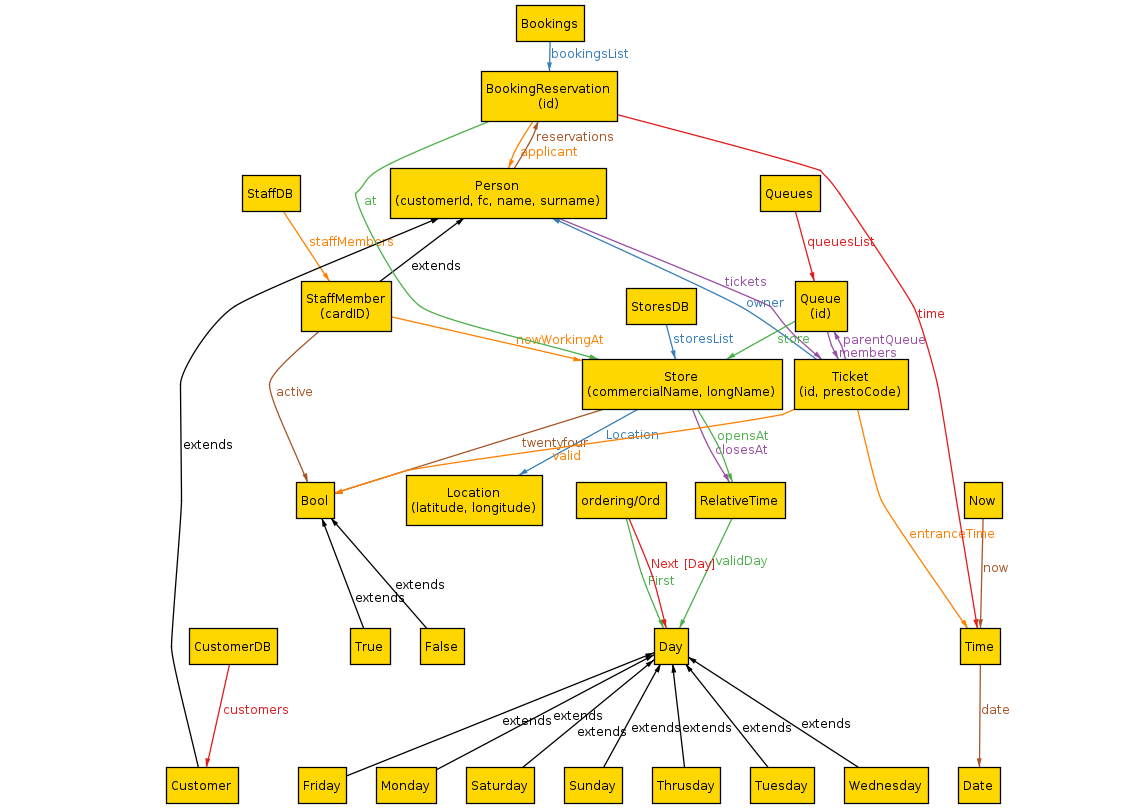
\includegraphics[width=\linewidth]{../Alloy/metamodel.png}
	\caption{The Alloy Metamodel}
	\label{fig:AlloyMainModel}
\end{figure}

\begin{figure} [H]
	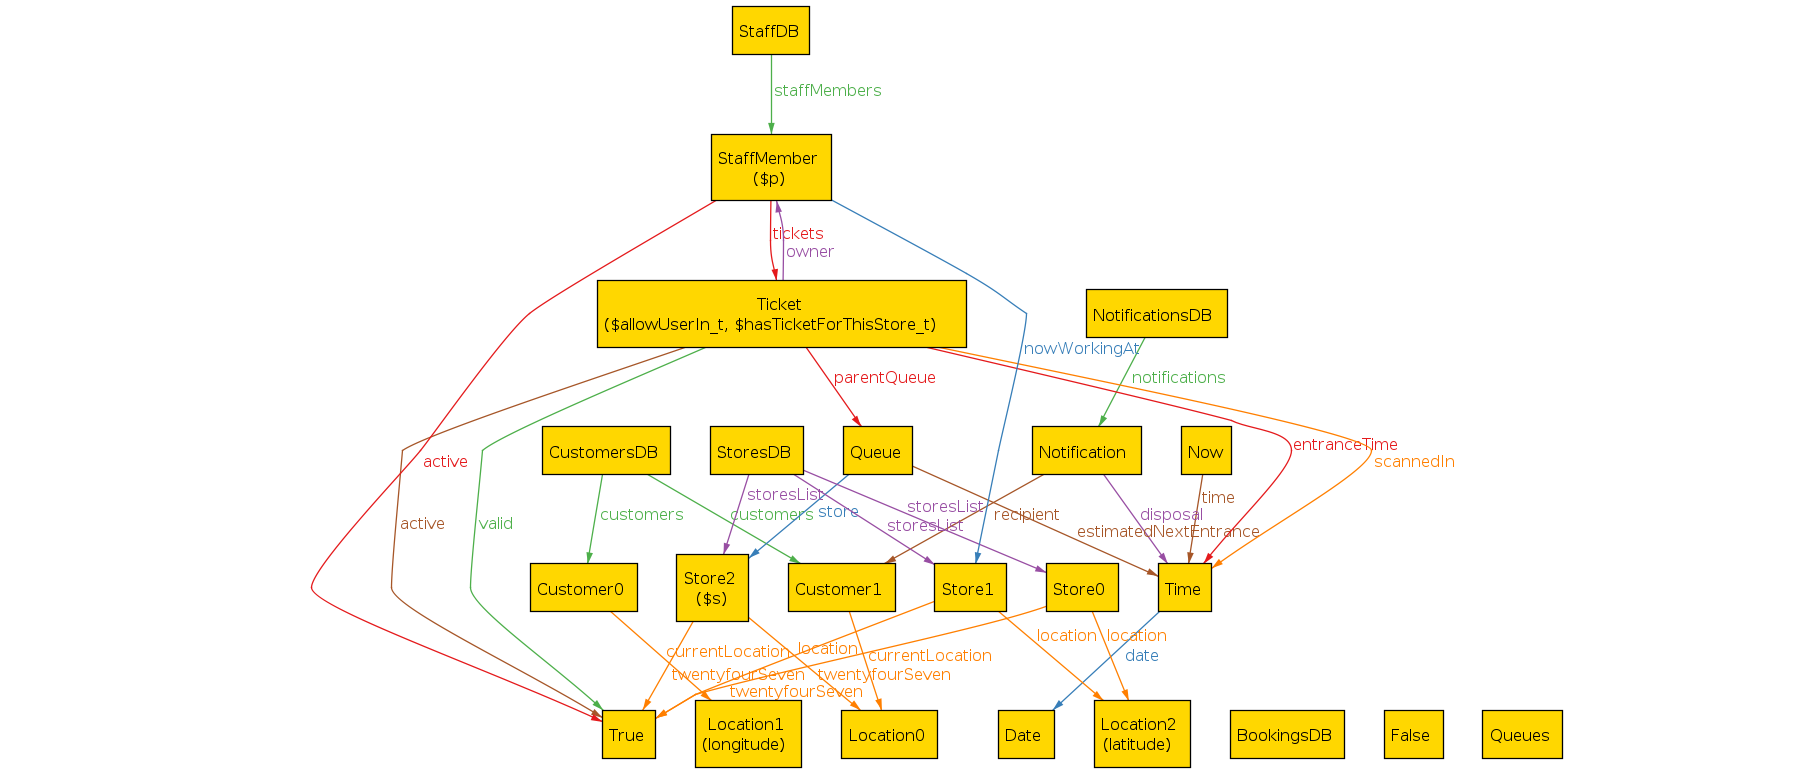
\includegraphics[width=\linewidth]{../Alloy/allowedInStaff.png}
	\caption{A staff member is allowed inside the store for shopping, hence being treated as a customer}
	\label{fig:allowedInStaff}
\end{figure}

\begin{figure} [H]
	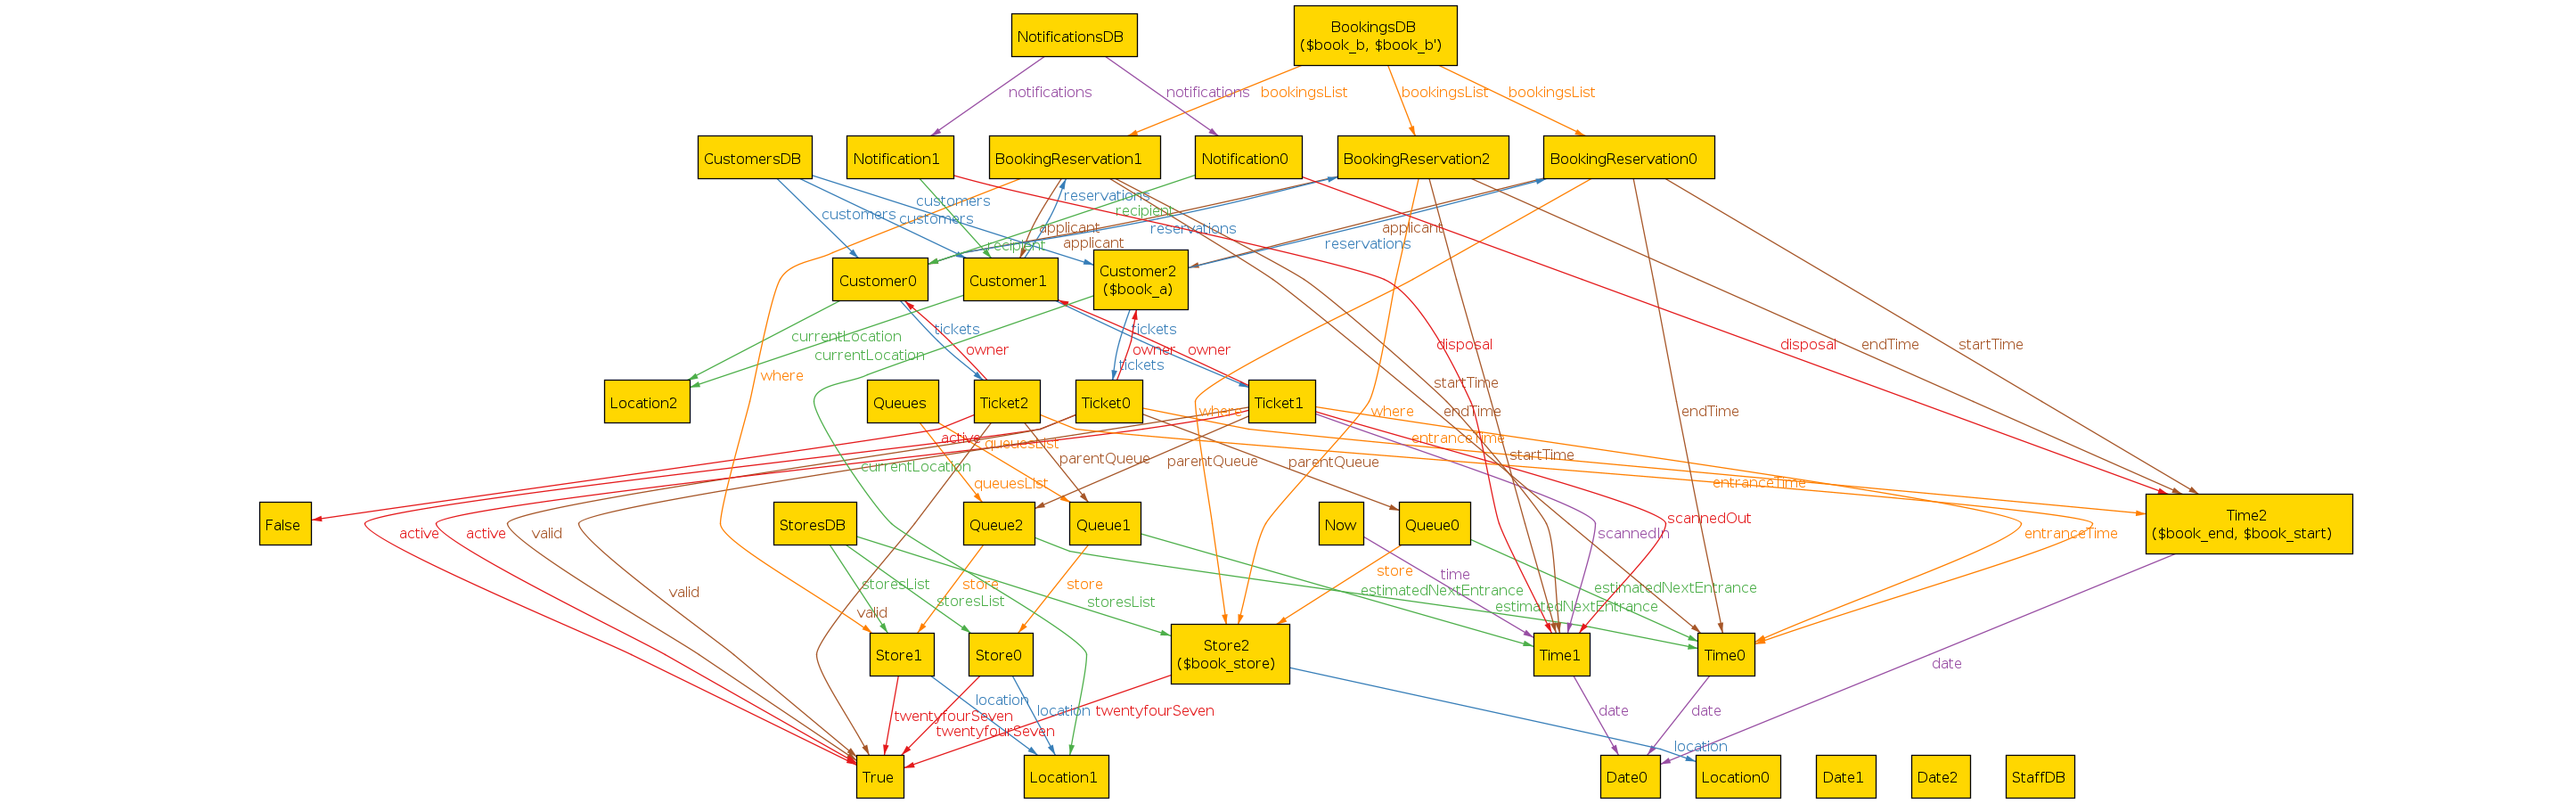
\includegraphics[width=\linewidth]{../Alloy/book.png}
	\caption{A booking procedure takes place}
	\label{fig:alloyBook}
\end{figure}

\begin{figure} [H]
	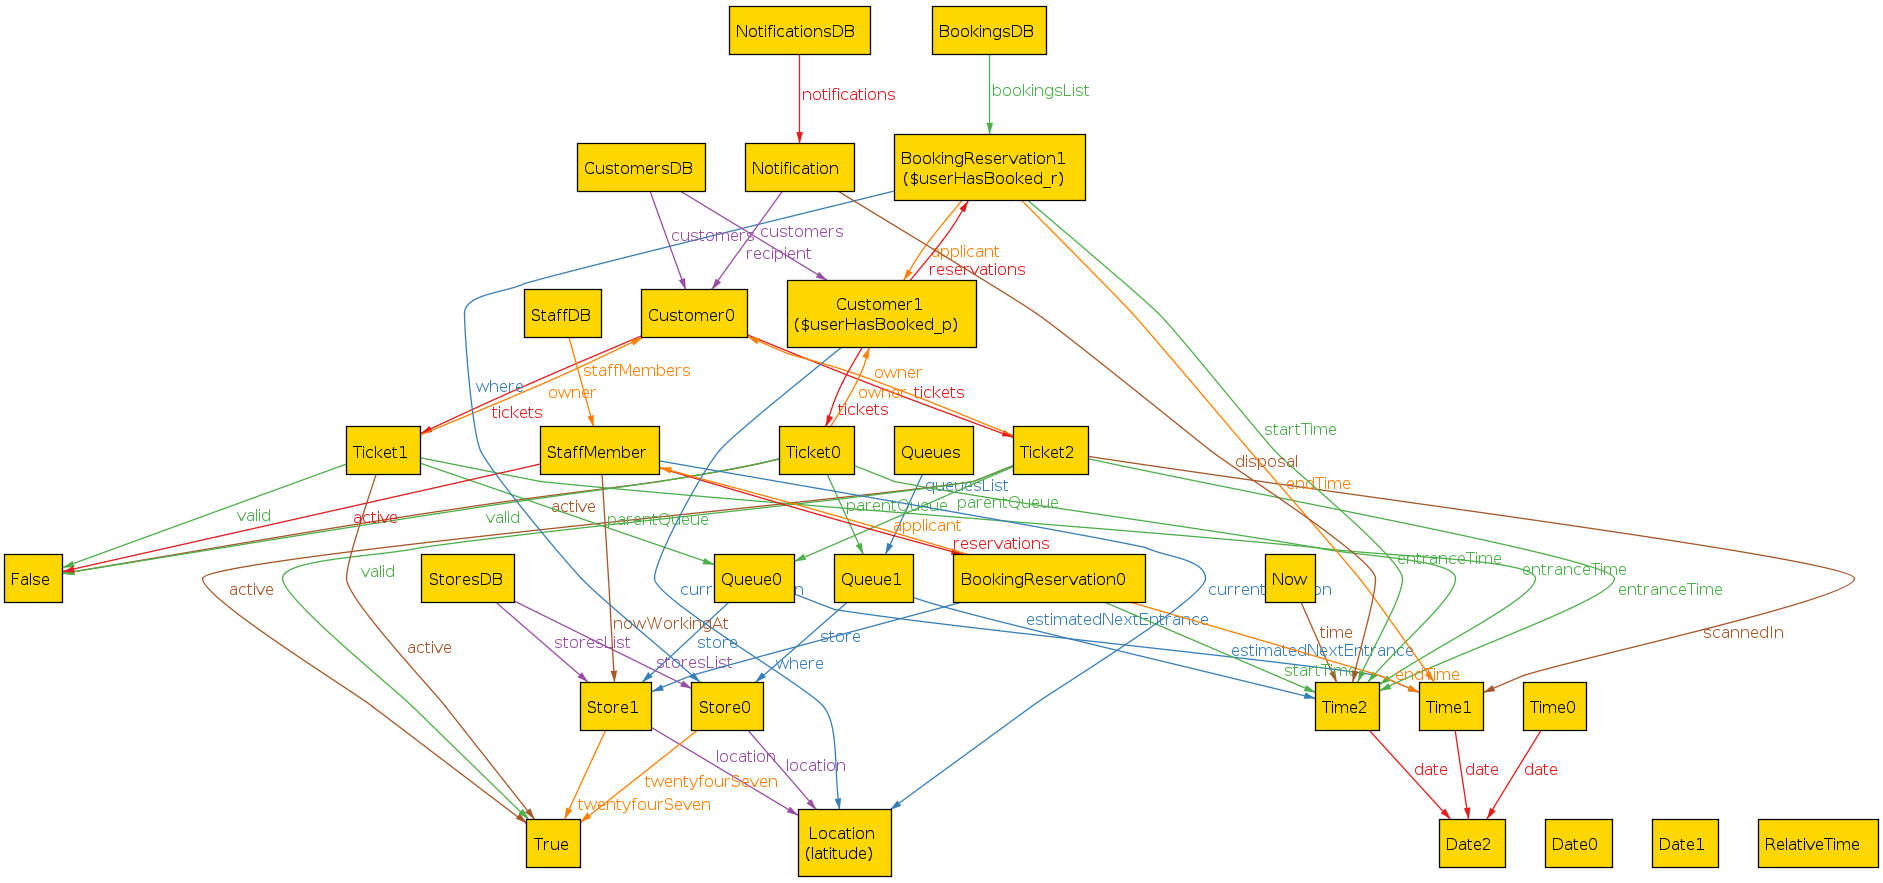
\includegraphics[width=\linewidth]{../Alloy/userHasBooked.png}
	\caption{User has made a reservation}
	\label{fig:userHasBooked}
\end{figure}

\begin{figure} [H]
	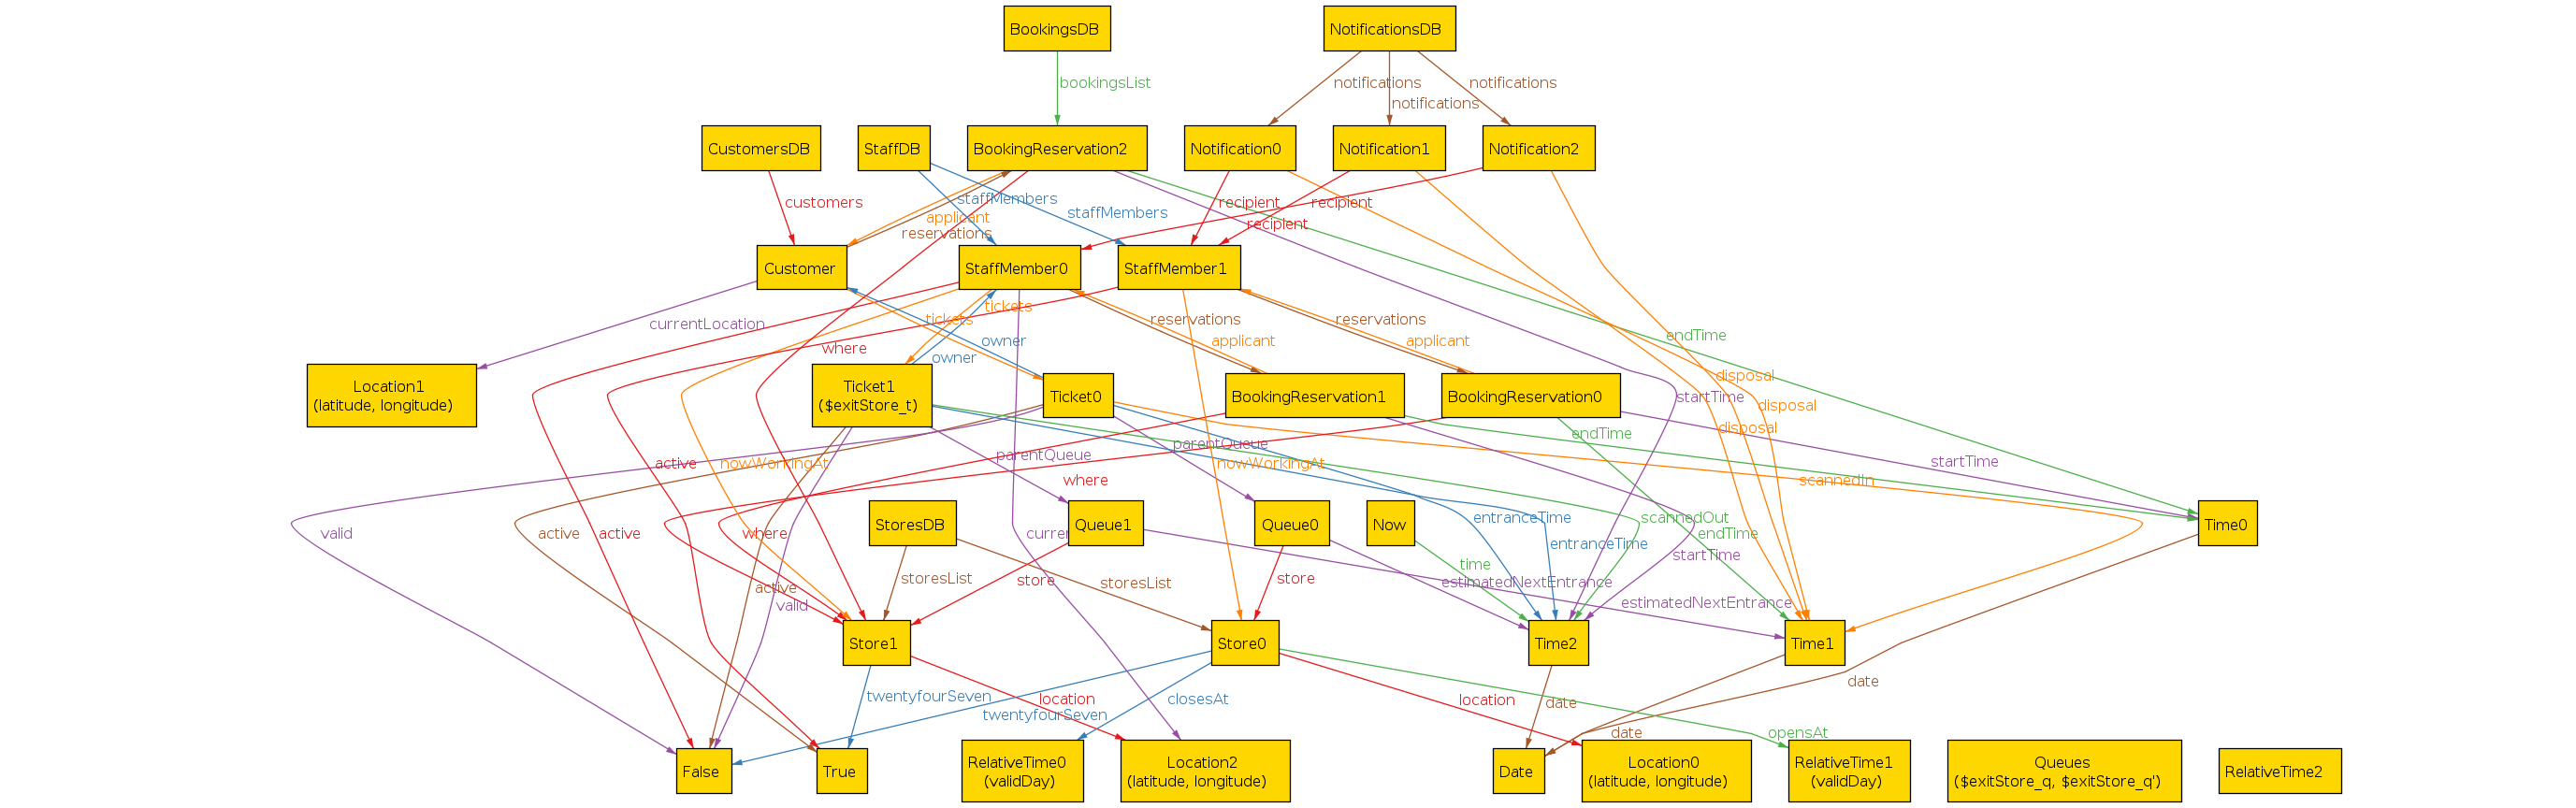
\includegraphics[width=\linewidth]{../Alloy/exitStore.png}
	\caption{User exits the store after shopping, causing ticket deletion}
	\label{fig:alloyExitStore}
\end{figure}

\begin{figure} [H]
	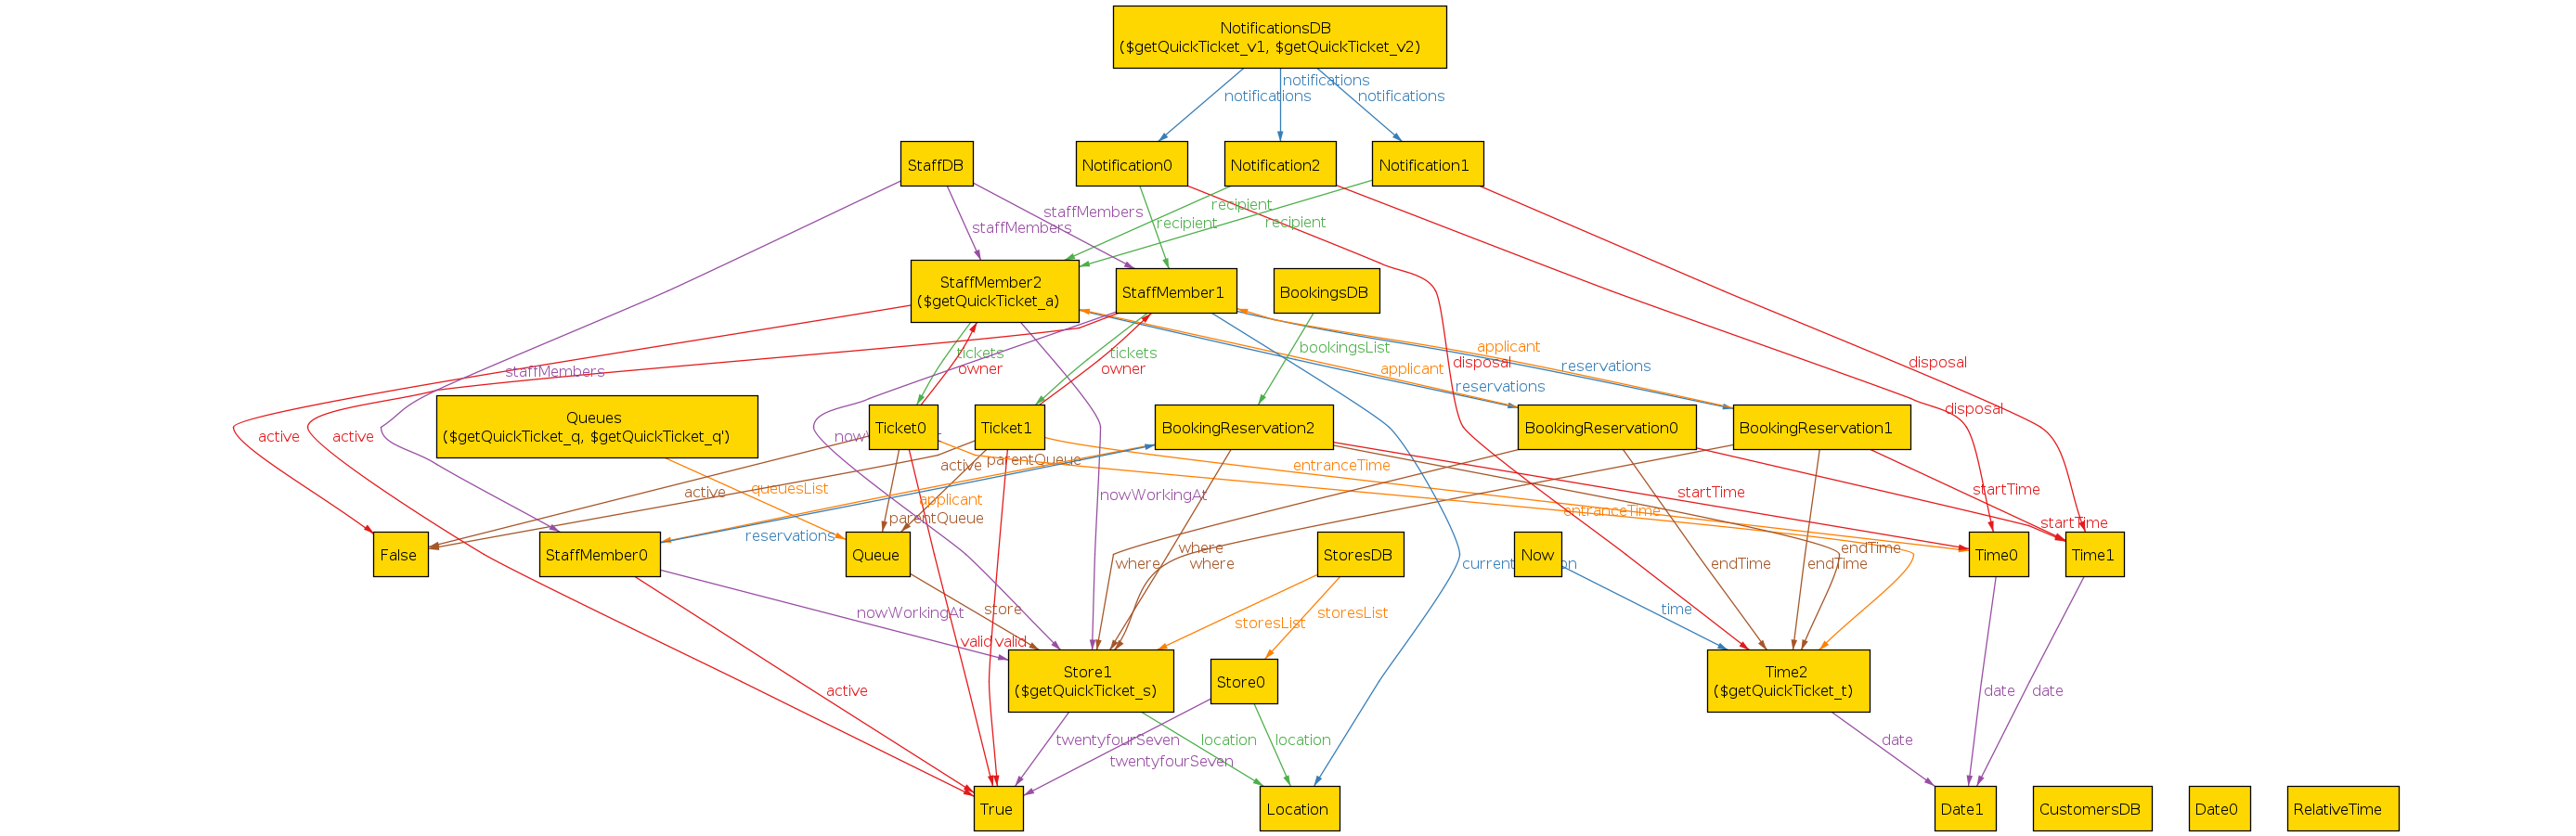
\includegraphics[width=\linewidth]{../Alloy/getQuickTicket.png}
	\caption{User gets a new quick ticket by using the mobile application}
	\label{fig:exitStore}
\end{figure}

\begin{figure} [H]
	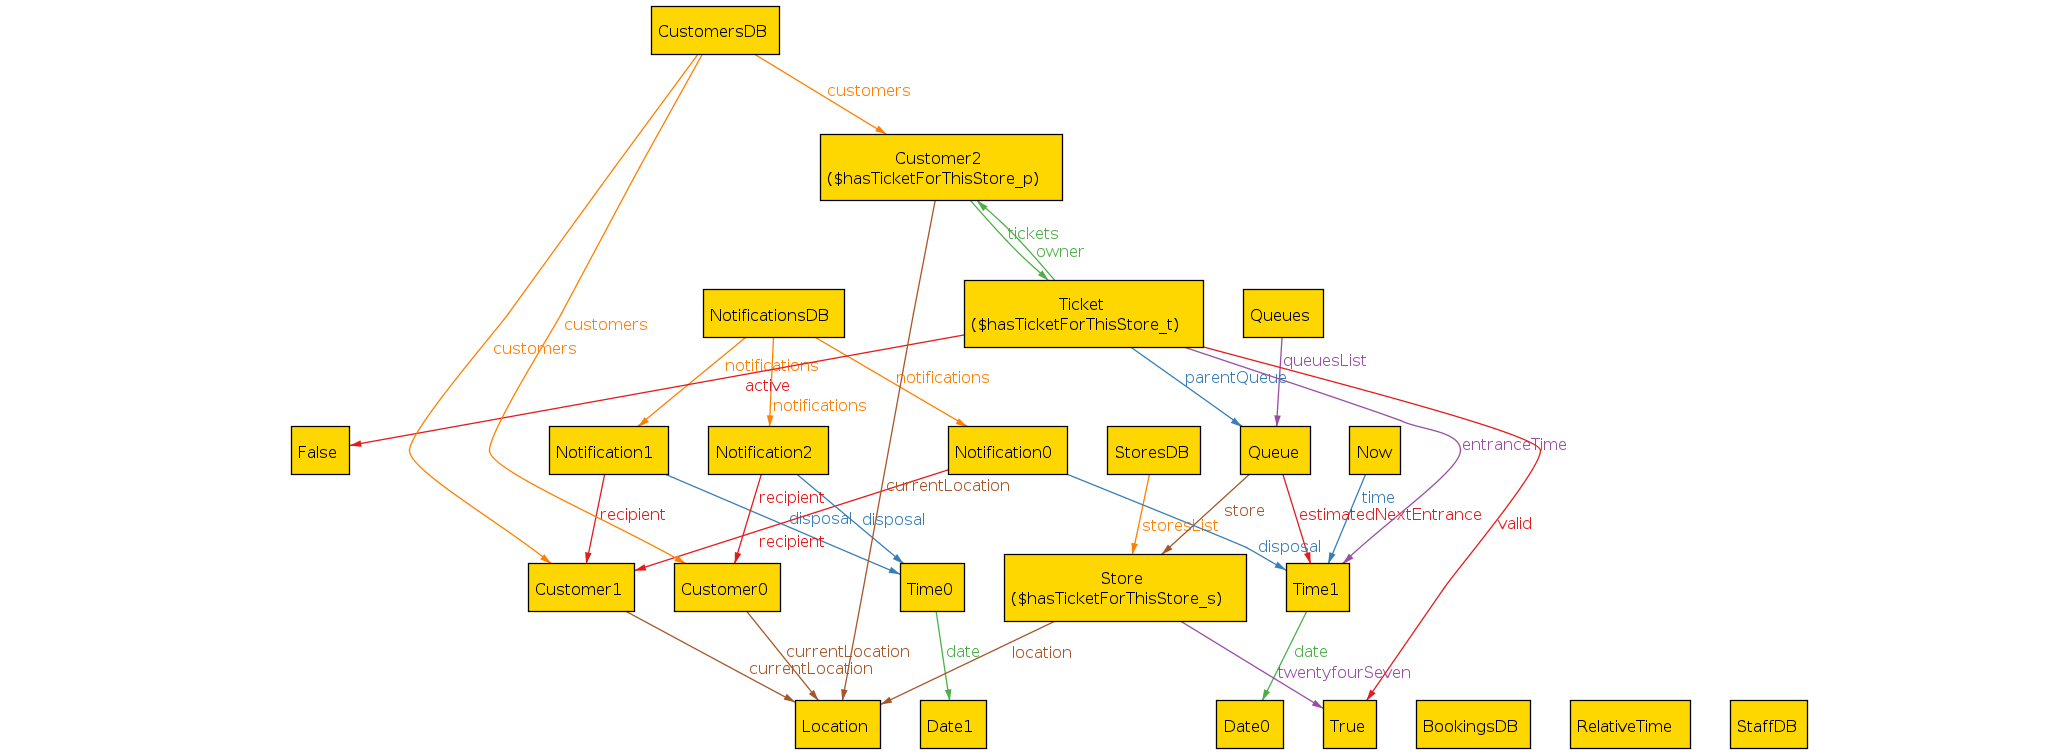
\includegraphics[width=\linewidth]{../Alloy/hasTicketForThisStore.png}
	\caption{User has a valid ticket for entrance}
	\label{fig:hasTicketForThisStore}
\end{figure}

\begin{figure} [H]
	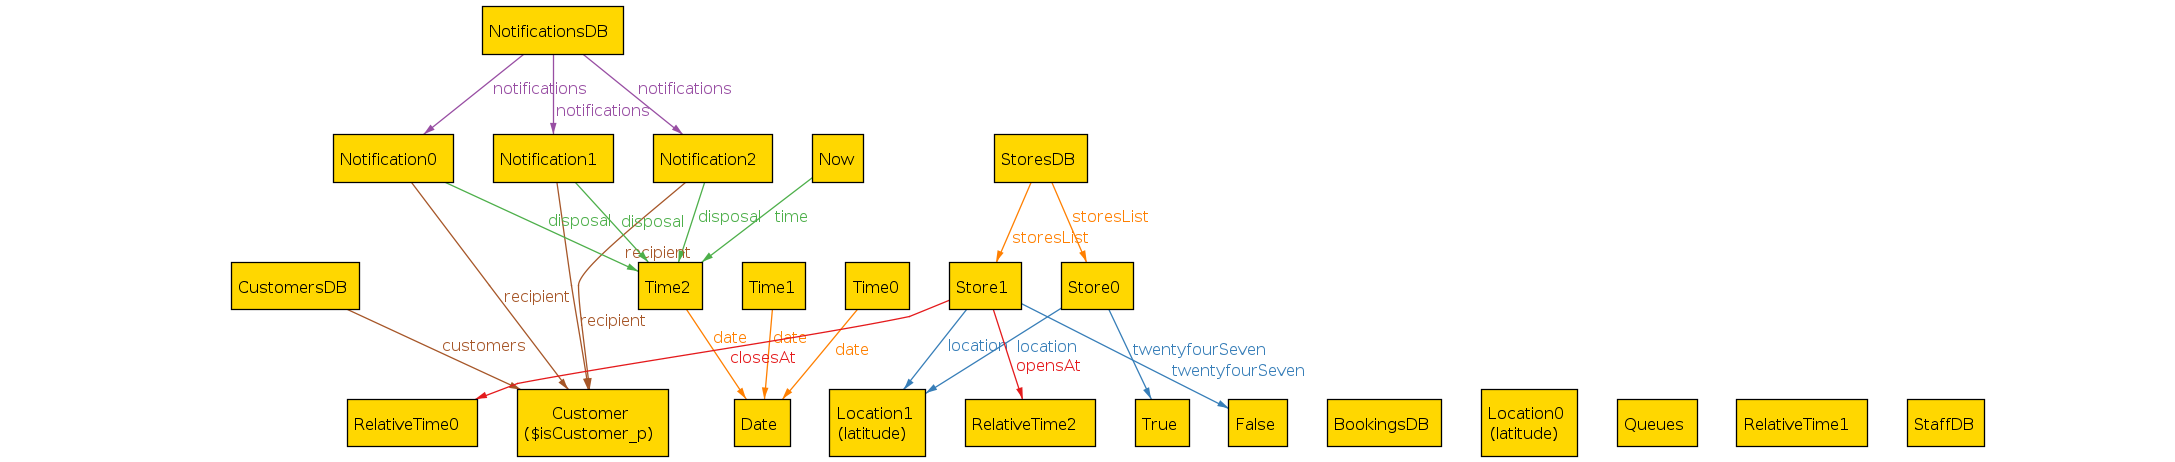
\includegraphics[width=\linewidth]{../Alloy/isCustomer.png}
	\caption{A new customer}
	\label{fig:alloyIsCustomer}
\end{figure}

\begin{figure} [H]
	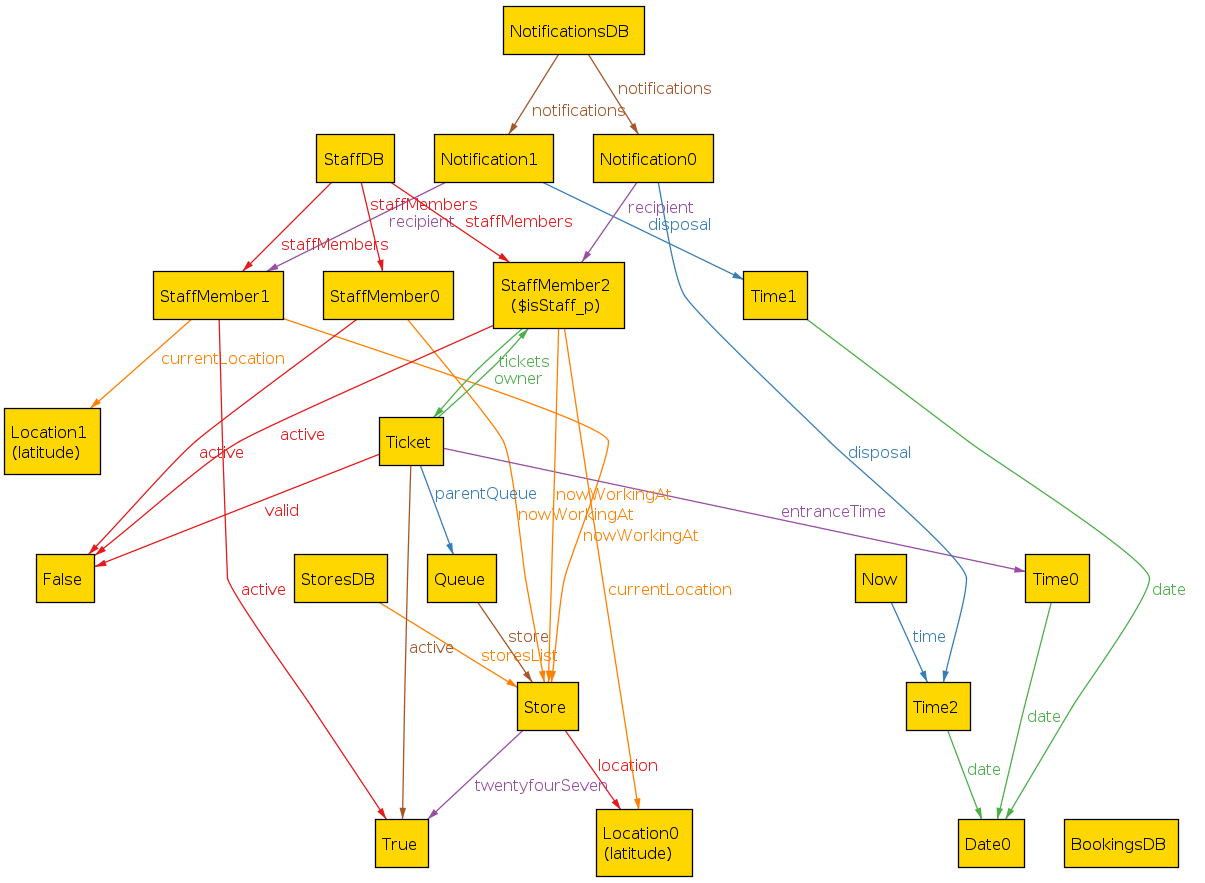
\includegraphics[width=\linewidth]{../Alloy/isStaff.png}
	\caption{A new staff member}
	\label{fig:alloyIsStaff}
\end{figure}

\begin{figure} [H]
	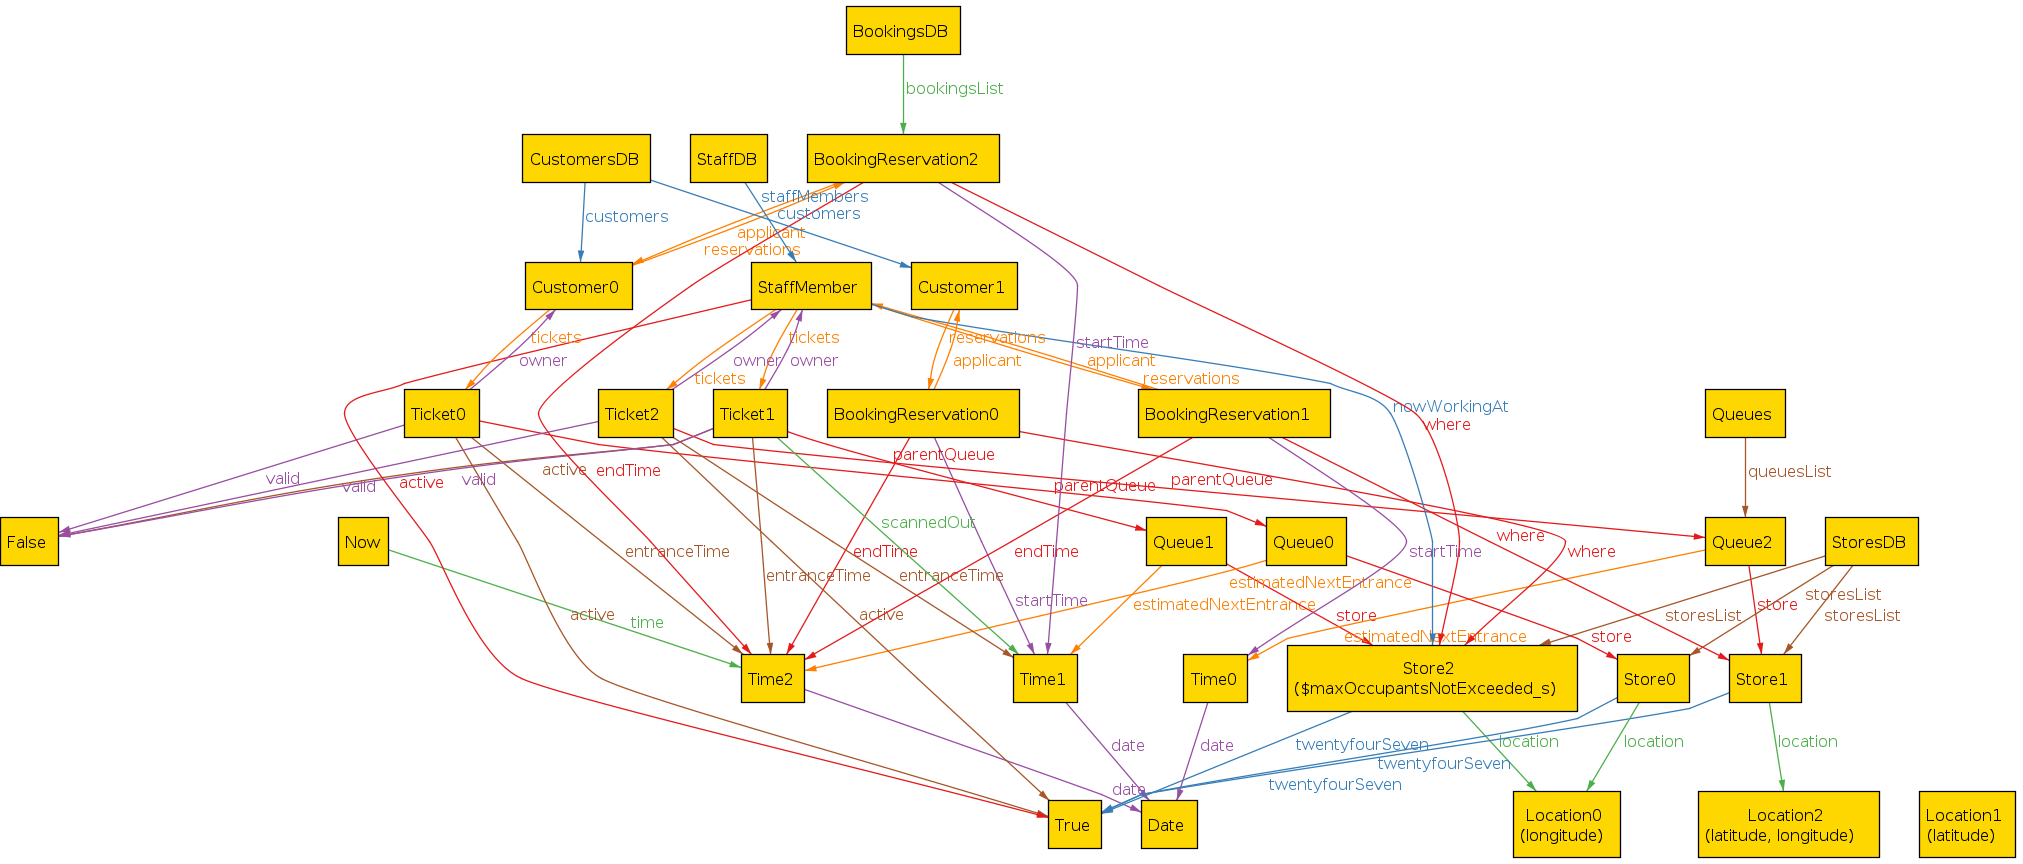
\includegraphics[width=\linewidth]{../Alloy/maxOccupantsNotExceeded.png}
	\caption{Showing it is possible not to exceed the max capacity of a store}
	\label{fig:maxOccupantsNotExceeded}
\end{figure}

\begin{figure} [H]
	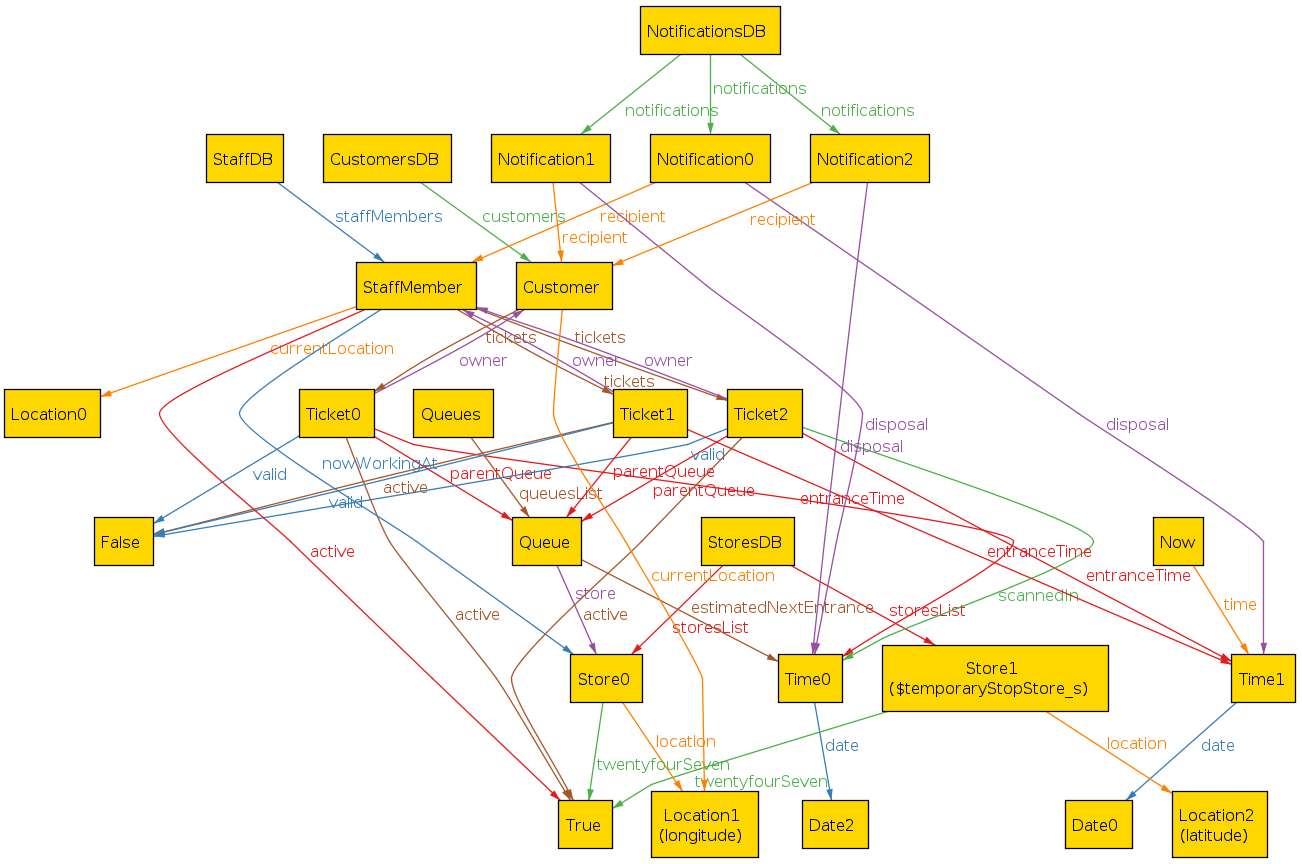
\includegraphics[width=\linewidth]{../Alloy/temporaryStopStore.png}
	\caption{Demonstrating the possibility of temporary interrupting store public access by the staff}
	\label{fig:temporaryStopStore}
\end{figure}

\subsection{Model test results}
The following extracts represent the results from testing the Alloy model with the automated tool.
\begin{figure} [H]
	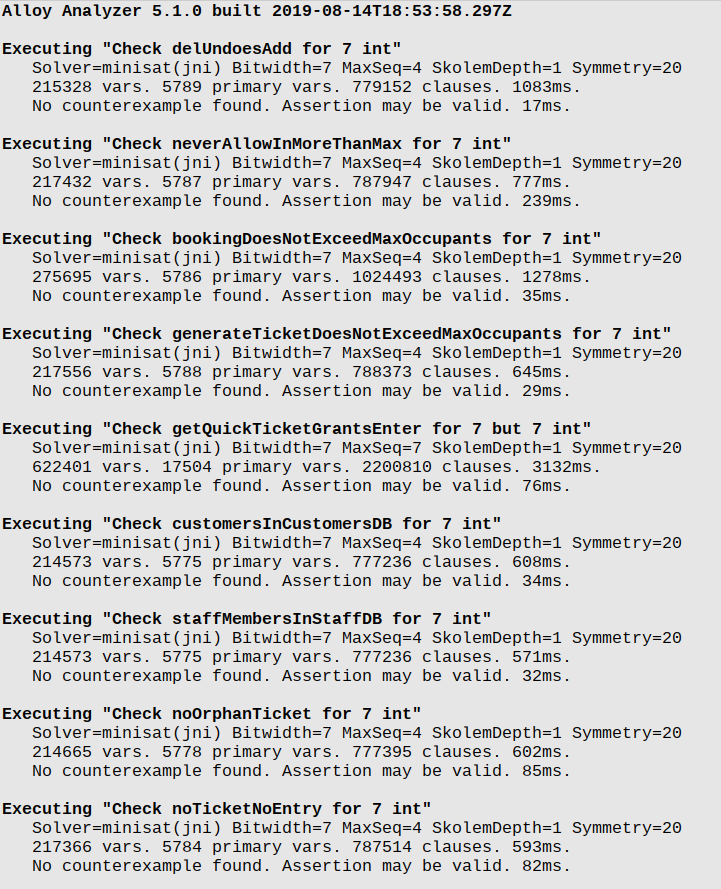
\includegraphics[width=\linewidth]{../Alloy/alloy_result1.png}
	\caption{Test results, part 1}
	\label{fig:results1}
\end{figure}
\begin{figure} [H]
	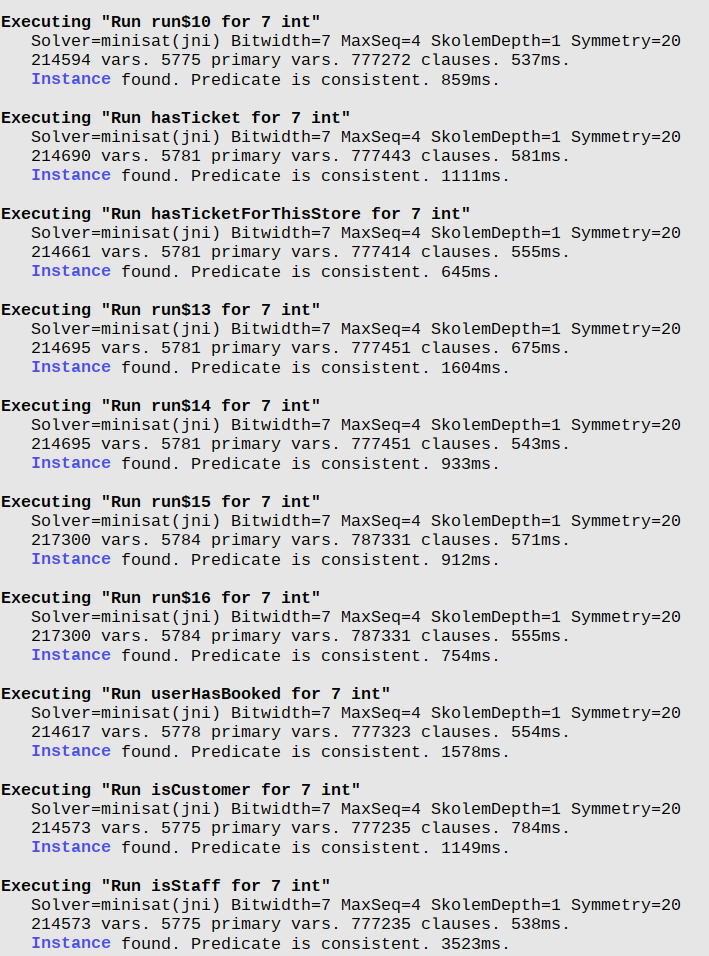
\includegraphics[width=\linewidth]{../Alloy/alloy_result2.png}
	\caption{Test results, part 2}
	\label{fig:results2}
\end{figure}
\begin{figure} [H]
	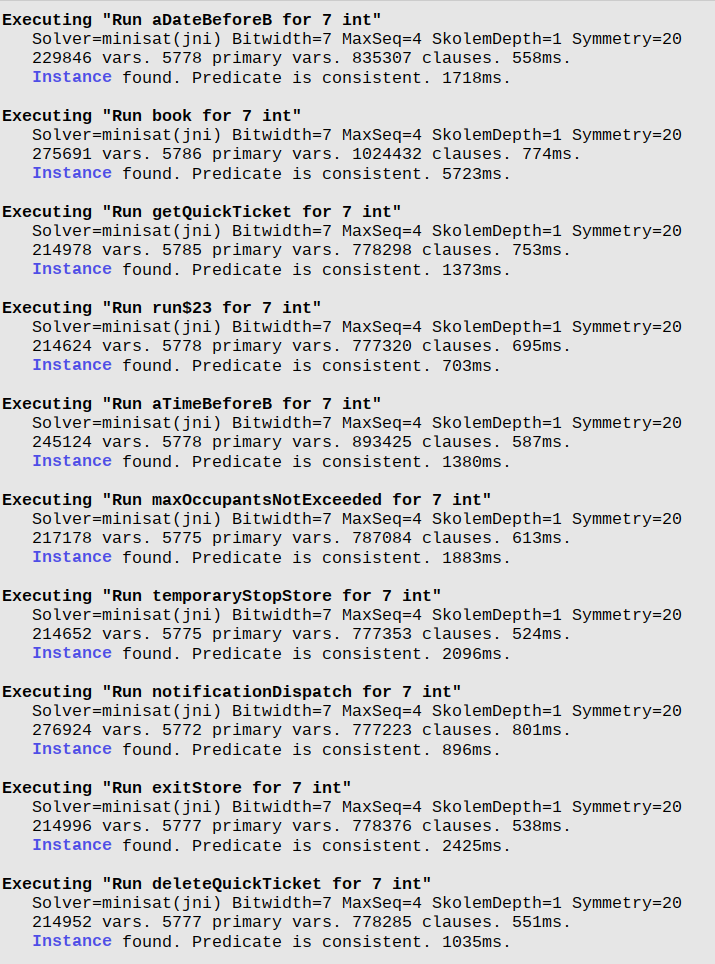
\includegraphics[width=\linewidth]{../Alloy/alloy_result3.png}
	\caption{Test results, part 3}
	\label{fig:results3}
\end{figure}
